%The MIT License (MIT)
%
%Copyright (c) 2018 Ronny Majani
%
%Permission is hereby granted, free of charge, to any person obtaining a copy
%of this software and associated documentation files (the "Software"), to deal
%in the Software without restriction, including without limitation the rights
%to use, copy, modify, merge, publish, distribute, sublicense, and/or sell
%copies of the Software, and to permit persons to whom the Software is
%furnished to do so, subject to the following conditions:
%
%The above copyright notice and this permission notice shall be included in all
%copies or substantial portions of the Software.
%
%THE SOFTWARE IS PROVIDED "AS IS", WITHOUT WARRANTY OF ANY KIND, EXPRESS OR
%IMPLIED, INCLUDING BUT NOT LIMITED TO THE WARRANTIES OF MERCHANTABILITY,
%FITNESS FOR A PARTICULAR PURPOSE AND NONINFRINGEMENT. IN NO EVENT SHALL THE
%AUTHORS OR COPYRIGHT HOLDERS BE LIABLE FOR ANY CLAIM, DAMAGES OR OTHER
%LIABILITY, WHETHER IN AN ACTION OF CONTRACT, TORT OR OTHERWISE, ARISING FROM,
%OUT OF OR IN CONNECTION WITH THE SOFTWARE OR THE USE OR OTHER DEALINGS IN THE
%SOFTWARE.

\documentclass{iyte}    %% main class file

% Caption Centering
% --------------
%\usepackage{caption}
 
%\captionsetup{justification=centering,singlelinecheck=false}

%\usepackage{graphicx}
\graphicspath{ {./images/} } 


% Using Hyperref
% --------------
%\usepackage[unicode]{hyperref}
%\hypersetup{
%	colorlinks   = true,    % Colours links instead of ugly boxes
%	urlcolor     = blue,    % Colour for external hyperlinks
%	linkcolor    = black,   % Colour of internal links; disabled for table of contents
%	citecolor    = black      % Colour of citations
%}


% Uncomment if you want to use the ACM Style References
% --------------
%\usepackage{url}
%\usepackage{natbib}




\begin{document}
\pagenumbering{roman}

% --------------

% Title Page Definitions
\thesistitle{AUTOMATIC, FAST AND ACCURATE SEQUENCE DECONTAMINATION}
\turkishthesistitle{OTOMAT\.{I}K, HIZLI VE DO\u{g}RU D\.{I}Z\.{I} DEKONTAM\.{I}NASYONU}
\thesisauthor{Ronny Majani}
\thesisdegree{MASTER OF Engineering}
\thesismajor{Computer Engineering}
\thesisdate{June}{2018}

% Add Title Page
\begin{titlepage}
	\newcommand*{\titlefont}[1]{\textbf{\fontsize{18pt}{27pt}\selectfont #1}}
	\newcommand*{\subtitlefont}[1]{\textbf{\setstretch{1}\fontsize{14pt}{21pt}\selectfont#1}}
	\begin{center}
		\vspace*{3em}  % 3 x single spacing
		\titlefont{
			\showthesistitle
		}
		
		\vspace{10em}
		\subtitlefont{
		A Thesis Submitted to\\
		the Graduate School of Engineering and Sciences of\\
		İzmir Institute of Technology\\
		in Partial Fulfillment of the Requirements for the Degree of\linebreak\\
		\showthesisdegree\linebreak\\%TODO: Fill with Correct Degree
		in \showthesismajor  %TODO: Fill with Correct Degree
		}
		
		\vspace{4em}
		
		\subtitlefont{
		by\\
		\showthesisauthor  %TODO: Fill with Student's Name
		}
		
		\vspace{7em}
		
		\subtitlefont{
			June 2018\\  %TODO: Fill with Correct Date
			İZMİR
		}
	\end{center}
\end{titlepage}
\addtocounter{page}{1}
\newpage

% --------------

% Signature Page Definitions
\signaturedate{10}{June}{2018}
\thesiscommitteememberA{Asst. Prof. Mustafa1}{Comp Eng}{IYTE}
\thesiscommitteememberB{Asst. Prof. Mustafa2}{Comp Eng}{IYTE}
\thesiscommitteememberC{Asst. Prof. Mustafa3}{Comp Eng}{IYTE}
\thesiscommitteememberD{Asst. Prof. Mustafa4}{Comp Eng}{IYTE}
\thesiscommitteememberE{Asst. Prof. Mustafa5}{Comp Eng}{IYTE}
\thesissupervisor{Asst. Prof. Mustafa Sup}{Comp Eng}{IYTE}
\thesiscosupervisor{Asst. Prof. Mustafa CoSup}{Comp Eng}{IYTE}
\thesisheadofdepartment{Asst. Prof. Mustafa Head}{Comp Eng}
\thesisdeanofgraduateschool{Asst. Prof. Mustafa De}

% Uncomment to manually set the vertical spacing of the signature page
% \setsignaturepagespacing{0.8cm}  % replace the argument with the desired value

% Add Signature Page
% Deine Macro for signature page

{\thispagestyle{empty}  % disable page numbering here
	We approve the thesis of \textbf{\showthesisauthor}\\
	
	\textbf{Examining Committee Members:}\\
	
	
	\ifdefined\showthesiscommitteememberA
		\showthesiscommitteememberA
	\fi
	
	\ifdefined\showthesiscommitteememberB
	\showthesiscommitteememberB
	\fi
	
	\ifdefined\showthesiscommitteememberC
	\showthesiscommitteememberC
	\fi
	
	\ifdefined\showthesiscommitteememberD
	\showthesiscommitteememberD
	\fi
	
	\ifdefined\showthesiscommitteememberE
	\showthesiscommitteememberE
	\fi
	
	\vspace{1.5em}
	\hfill
	\textbf{\showsignaturedate}
	\vspace{1.5em}
	
	\showthesissupervisor
	\showthesiscosupervisor
	
	\showthesisheadofdepartment
	\showthesisdeanofgraduateschool
}



%\begin{minipage}{7cm}%
%	\vspace{1.0cm}\namesigdatehrule{7cm}\smallskip
%	\noindent{
%			Asst. Prof. Mustafa Özuysal\\
%			Department of Computer Engineering, Izmir Institute of Technology
%		}
%\end{minipage}
\newpage

% --------------

\begin{dedication}
	I love family?
\end{dedication}

\begin{acknowledgments}
	I love life
\end{acknowledgments}

\begin{preface}
	Life is hard
\end{preface}

\begin{abstract}
	Fill in your abstract
\end{abstract}

\begin{ozet}
	Burada bir \"{o}zet yaz
\end{ozet}

\tableofcontents
\newpage
\listoffigures
\newpage
\listoftables
\newpage


\chapter{Introduction}
\pagenumbering{arabic}

\section{life}
life

\subsection{more life}
life

\subsubsection{even more life}
aaaa

\subsubsubsection{mini life}  % equivalent to \paragraph{mini life}
bb

\subsubsubsubsection{tiny life} % equivalent to \subparagraph{tiny life}
yay

Text text text text text text text text text text
\begin{equation}
1 + 2 + 3 = 6
\end{equation}  
\begin{equation}
1 + 2 + 3 = 6
\end{equation} 
\begin{equation}
1 + 2 + 3 = 6
\end{equation} 

Text text text text text text text text text text
\begin{align}
1 + 2 + 3 &= 6 \\
1 + 2 + 3 &= 6
\end{align}



Text text text text text text text text text text
\begin{equation}
1 + 2 + 3 = 6
\end{equation}  
Text text text text text text text text text text
\begin{align}
1 + 2 + 3 &= 6 \\
1 + 2 + 3 &= 6
\end{align}

\begin{figure}[h]
	\caption{Very cute cat}
	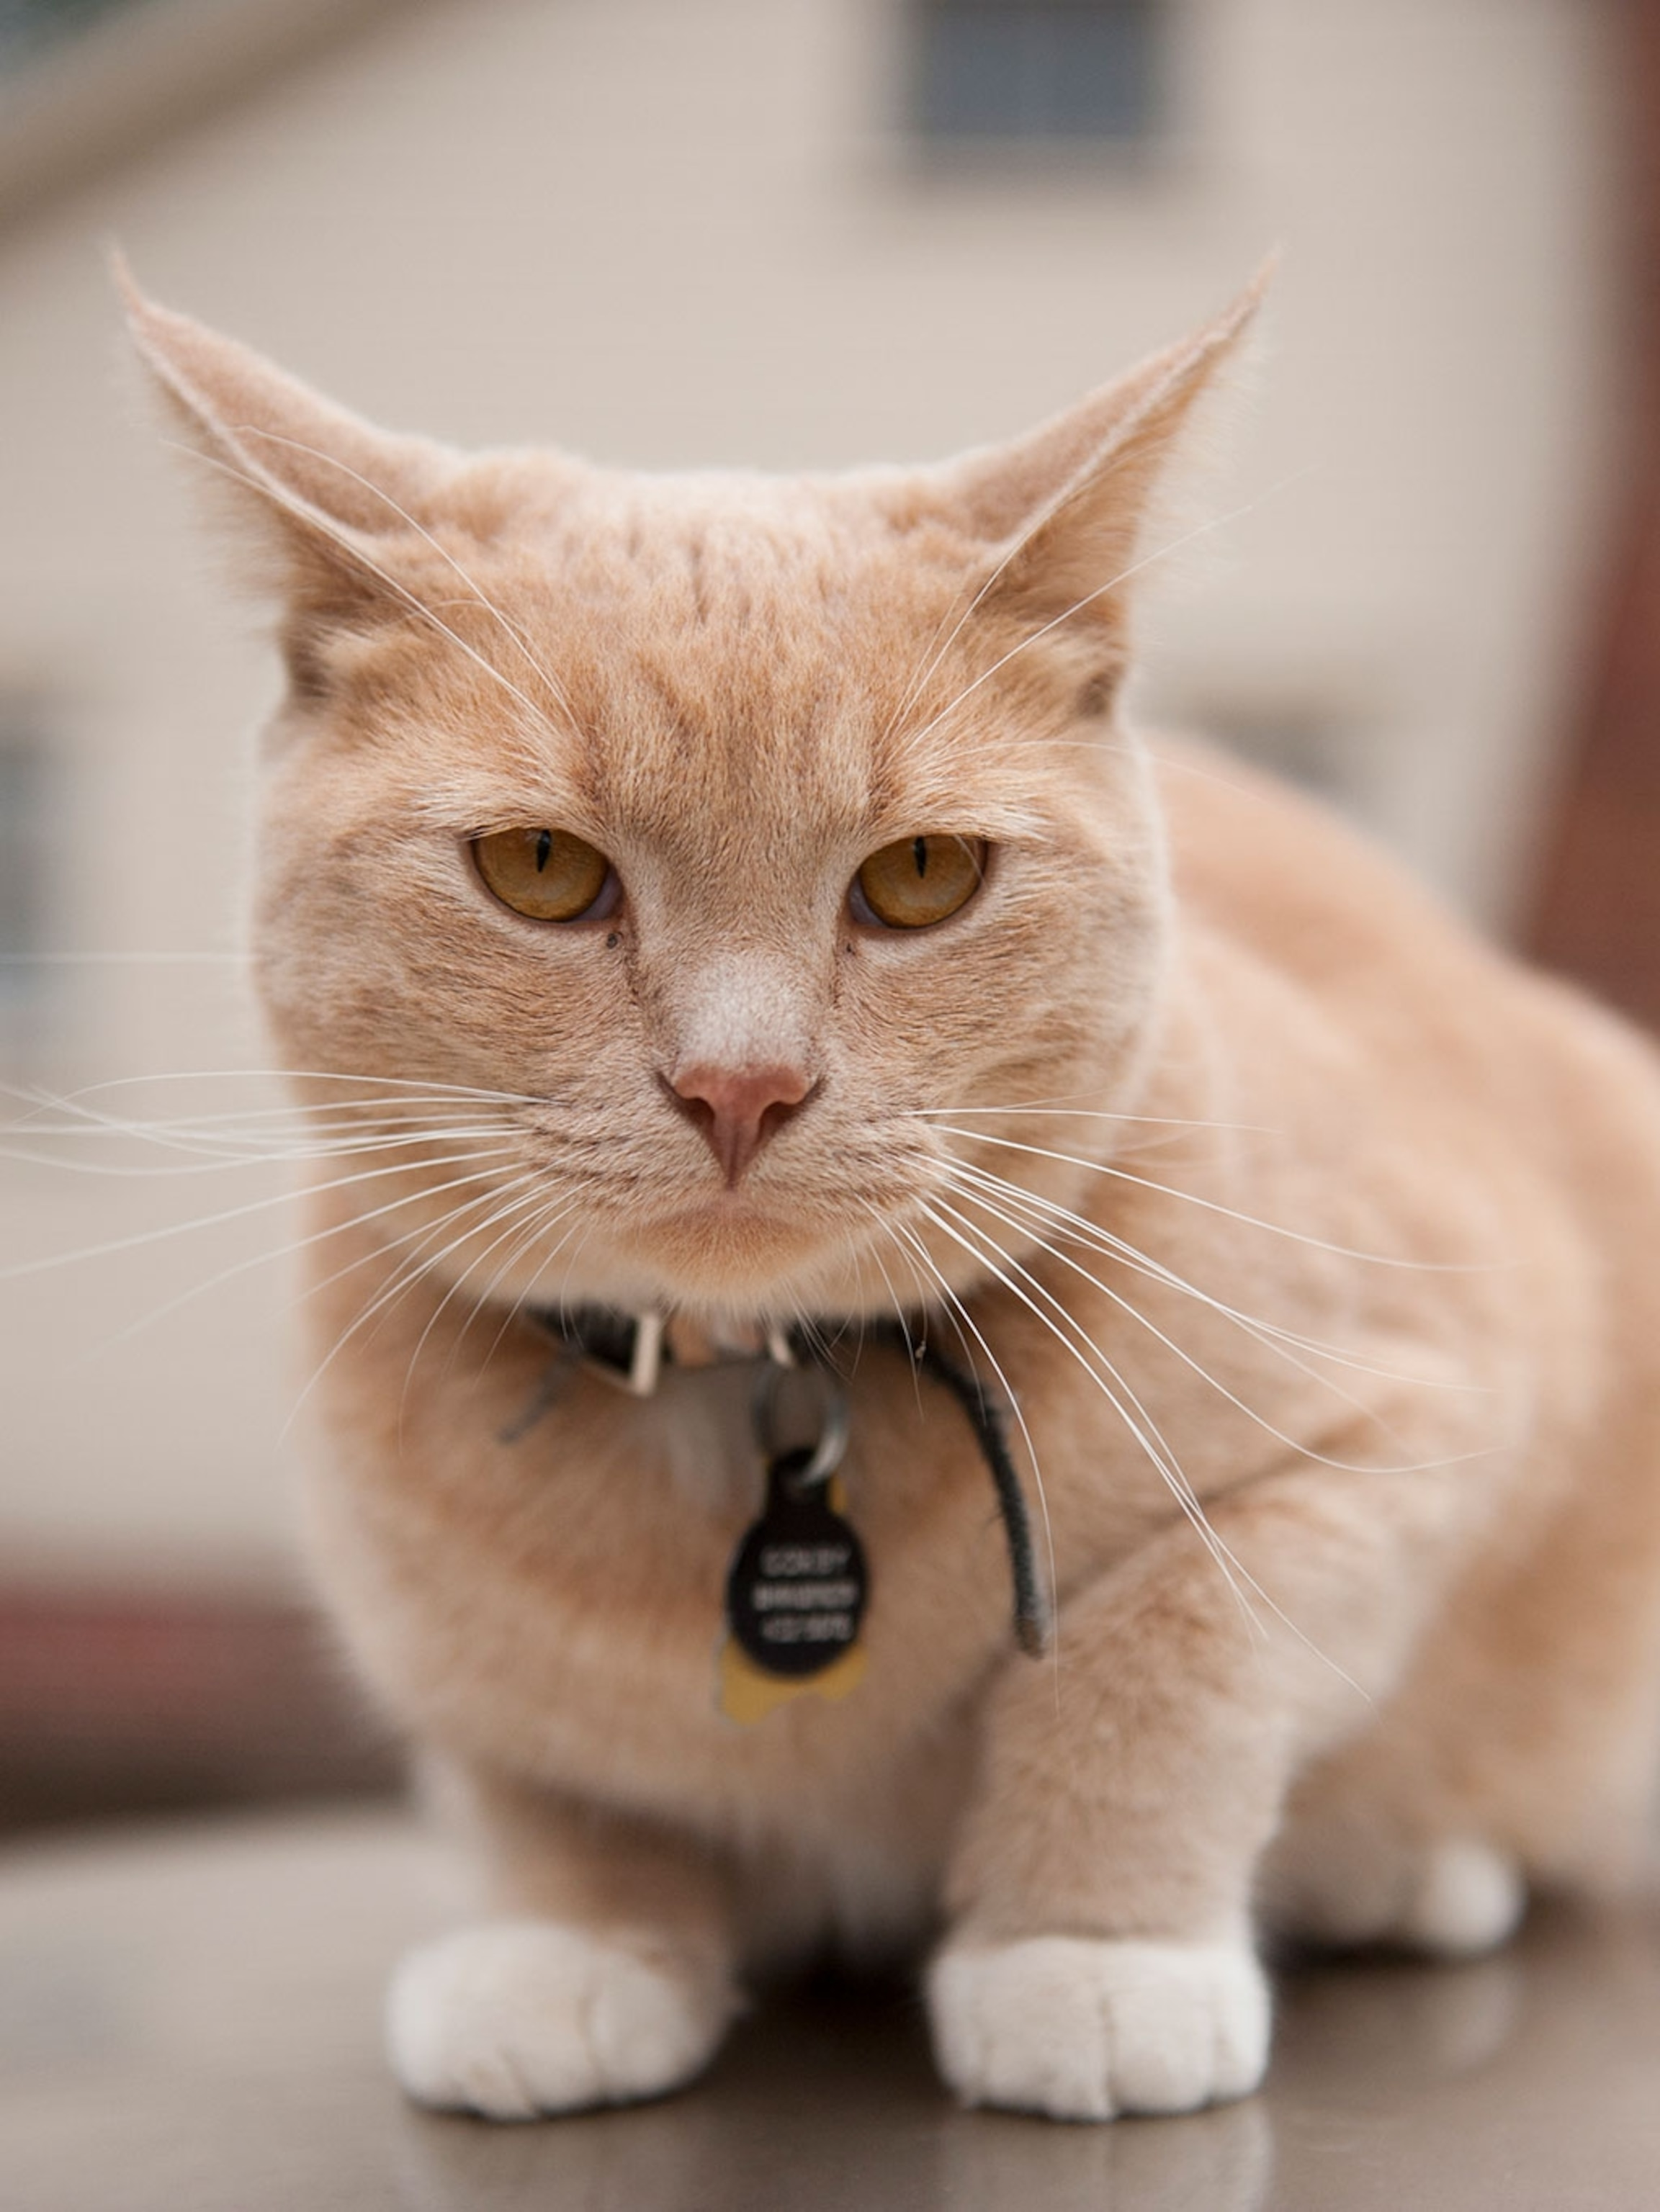
\includegraphics[width=200px]{cat}
	\centering
\end{figure}

\begin{table}[h!]
	\centering
	\caption{A really cool table}
	\begin{tabular}{||c c c c||} 
		\hline
		Col1 & Col2 & Col2 & Col3 \\ [0.5ex] 
		\hline\hline
		1 & 6 & 87837 & 787 \\ 
		\hline
		2 & 7 & 78 & 5415 \\
		\hline
		3 & 545 & 778 & 7507 \\
		\hline
		4 & 545 & 18744 & 7560 \\
		\hline
		5 & 88 & 788 & 6344 \\ [1ex] 
		\hline
	\end{tabular}
\end{table}


\begin{thesisappendices}
	\chapter{Misc}
	The contents...
	\chapter{Other Stuff}
	More weird contents...
\end{thesisappendices}


% Uncomment to enable ACM style References:
% --------------
%\bibliographystyle{ACM-Reference-Format}
%\bibliography{references}

\end{document}
